% =====================================================================
%  From Datasheet to Diagnosis
%  Ethics in Artificial Intelligence, McGill University, Final Paper
%  Compile on Overleaf with pdfLaTeX. Upload the folder "figures/" too.
%
%  FINAL VERSION 2.
%
%  PAGE BUDGET. The brief allows 10 pages excluding the cover page and the
%  references. Version 1 put the abstract and a contributions box on their own
%  sheet and treated them as front matter; a teaching assistant advised that
%  both would be counted, so there is no separate abstract page here. What the
%  abstract said has been folded into the Introduction, where the contributions
%  also now live, and the method diagram that readers found most useful is
%  Figure 1 rather than an appendix item. Introduction through Conclusion must
%  fit in 10 pages. The weakest results -- the preregistered hypothesis tests,
%  which are mostly unresolved, and the corpus non-identifiability argument --
%  were moved to the appendix to pay for it, and the body points at them.
% =====================================================================
\documentclass[11pt,twocolumn]{article}

\usepackage[T1]{fontenc}
\usepackage[utf8]{inputenc}
\usepackage{newtxtext,newtxmath}
\usepackage[margin=0.85in]{geometry}
\setlength{\columnsep}{18pt}
\usepackage{graphicx}
\usepackage{booktabs}
\usepackage{tabularx}
\usepackage{array}
\usepackage[table]{xcolor}
\usepackage{caption}
\usepackage{subcaption}
\usepackage{enumitem}
\usepackage{longtable}
\usepackage{microtype}
\usepackage{cite}
\usepackage[colorlinks=true,linkcolor=darkred,citecolor=darkred,urlcolor=darkred]{hyperref}

\definecolor{darkred}{HTML}{8B0000}
\definecolor{rose}{HTML}{F8EBEB}
\definecolor{redt}{HTML}{FBE2DF}

\captionsetup{font=footnotesize,labelfont=bf,skip=3.5pt}

% Float placement. LaTeX's defaults reserve so much of a page for text that a
% float-heavy document leaves half-empty pages: before this, six pages ran 37-46
% lines against 101 on a full one. These let a float take more of a page and a
% page hold more floats, which is what keeps the body inside the limit.
\renewcommand{\topfraction}{0.92}
\renewcommand{\bottomfraction}{0.85}
\renewcommand{\textfraction}{0.06}
\renewcommand{\floatpagefraction}{0.80}
\setcounter{topnumber}{3}
\setcounter{bottomnumber}{2}
\setcounter{totalnumber}{5}
\setlength{\textfloatsep}{10pt plus 2pt minus 3pt}
\setlength{\intextsep}{9pt plus 2pt minus 3pt}
\setlength{\floatsep}{8pt plus 2pt minus 3pt}
\setlist{itemsep=1pt,topsep=3pt,parsep=0pt}
\renewcommand{\arraystretch}{1.0}
\newcolumntype{L}{>{\raggedright\arraybackslash}X}
\linespread{0.975}
\graphicspath{{figures/}}

\begin{document}

% ------------------------------------------------------------------ cover
\begin{titlepage}
\centering
\vspace*{1.6cm}
{\color{darkred}\rule{\linewidth}{1.2pt}}\\[0.5cm]
{\LARGE\bfseries From Datasheet to Diagnosis\par}
\vspace{0.35cm}
{\Large Tracing gender bias through open training-data pipelines\\into the health advice of large language models\par}
\vspace{0.35cm}
{\color{darkred}\rule{\linewidth}{1.2pt}}\\[1.3cm]
{\large Evans Kumi \quad and \quad Aymen Boustani\par}
\vspace{0.3cm}
{\large M.Sc.\ Intelligent Systems\par}
\vspace{0.18cm}
{\large Department of Electrical, Computer and Software Engineering, McGill University\par}
\vspace{0.9cm}
{\large Final paper\;\textbullet\; Ethics in Artificial Intelligence\;\textbullet\; November 2026\par}

\vspace{0.95cm}
% D133. The abstract and the contributions live HERE, on the cover page, not
% in the body. A teaching assistant warned that an abstract and a contributions
% section would be counted inside the 10 pages; one cover page is excluded by
% the brief, so this keeps both without spending body space. The acknowledgement
% that used to sit here is now at the end of the appendix.
\begin{minipage}{0.95\linewidth}
\footnotesize
\setlength{\tabcolsep}{7pt}
\renewcommand{\arraystretch}{1.2}
\begin{tabularx}{\linewidth}{@{}p{2.05cm}L@{}}
\toprule
\textbf{\color{darkred}Abstract} &
Large language models already answer health questions, and audits show they can
treat women and men differently when the clinical facts are identical. Those
audits cannot say \emph{why}, because the training data of the models they test
is closed. We use the two families whose data is public, Pythia on the Pile and
OLMo~2 on OLMo-mix, to audit three things on one scale: gender skew in the
training data, gender gaps in the models' clinical answers, and what the dataset
documentation says about either. We wrote 25 clinical vignettes, short written
patient cases of the kind used to examine medical students, each with a correct
answer quoted from a named clinical guideline, and expanded them into 624
prompts that vary the patient's gender identity while holding fixed the sex
parameter a guideline actually reasons over. Ten models were scored against two
measured noise floors and a positive control. \\
\midrule
\textbf{\color{darkred}Contributions} &
\textbf{1. A positive control for clinical fairness audits.} Group~2, where the
guideline's own answer changes with the sex parameter, so a model whose answer
does not shift there cannot be read anywhere else. \textbf{7 of 10 fail it},
which makes their small gender gaps blindness rather than fairness.
\newline
\textbf{2. A placebo floor on the same vignette.} An effect must also beat a
clinically inert edit to the identical case, not a gender flip on a different
one. This takes the interpretable set \textbf{from 3 of 10 to 0 of 10}.
\newline
\textbf{3. Sex and gender held apart in the prompt.} Every model capable enough
to audit reads the identity label \emph{as} the sex parameter, by up to
\textbf{21.5 times its own noise floor}: the configuration of a transgender
patient. Instruction tuning on identical data more than tripled it.
\newline
\textbf{4. Two findings that need no model.} ``The non-binary patient'' occurs
\textbf{zero times} in either open corpus, and the OLMo-mix dataset card never
mentions gender while the Pile measured it, so disclosure is a choice rather
than a property of being open. \\
\bottomrule
\end{tabularx}
\end{minipage}

\vfill
\vspace{0.7cm}
{\footnotesize\itshape Keywords: algorithmic fairness, clinical decision support,
training-data transparency, datasheets, gender bias, large language models.\par}
\vspace{0.5cm}
{\footnotesize This cover page, the references and the appendix are excluded from
the 10-page limit. The report body runs from page~1 to page~10.\par}
\end{titlepage}

% There is no separate abstract page in this version. What it carried is in the
% Introduction: the problem, then the method, then the four results, which are
% also the contributions. Arabic numbering starts at the Introduction.
\twocolumn
\pagenumbering{arabic}
\setcounter{page}{1}

% =====================================================================
\section{Introduction}
% =====================================================================

Clinical medicine has always depended on who is believed. Whose pain is treated
as real, whose breathlessness is investigated and whose account of their own body
is taken at face value are decisions made by people, and decades of evidence show
those decisions have not been made evenly~\cite{r18,r19,r20}. What is new is that
the decisions are starting to be made, or at least shaped, by software. People
ask chatbots about their symptoms before they call a clinic, and hospitals are
piloting language models for triage, summarisation and decision support. A
difference that a single clinician applies to a handful of patients is a personal
failing; the same difference inside a model applied to millions of queries is a
policy, enacted at scale and with the appearance of neutrality.

That makes it an ethics problem rather than only an engineering one, and it
raises a question of evidence: how would anyone know? Zack et al.\ showed the
risk is real, finding that GPT-4 changed its diagnoses and management plans with
the patient's stated gender and race on otherwise identical cases~\cite{r12}.
The case that motivated this project is a patient with a pulmonary embolism, a
life-threatening clot in the lungs, described to a model that offers a panic
attack instead. Attributing women's physical symptoms to emotion is one of the
best-documented biases in human medicine~\cite{r18,r20}, and here a machine has
reproduced it.


Audits of this kind stop at the output for a structural reason: the data
commercial models are trained on is a trade secret, so the only observable is
the answer. The strongest available finding is therefore
``this model is biased'', which supports no particular action. By contrast,
``this model is biased, the bias is present in its training data, and the
documentation never warned anyone'' supports three: fix the data, require the
disclosure, or decline to deploy. Moving from the first sentence to the second is
the purpose of this paper.

A small number of model families make that move possible by publishing their full
training data. Pythia is trained on the Pile~\cite{r6,r17} and OLMo~2 on
OLMo-mix~\cite{r7,r8}, and both corpora can be searched for exact phrases through
infini-gram~\cite{r9}. For these models, and almost no others, data and behaviour
can be put on one scale. We therefore ask
whether gender skew in open training data appears as clinically unwarranted
gender differences in model health advice, and whether the documentation of that
data disclosed the risk. 

This breaks into six questions. The \emph{data audit} asks whether there is a measurable gender skew around health concepts in the open corpora, and whether non-binary patients are represented at all (RQ1). The \emph{output audit} asks whether the models produce gender gaps that no guideline warrants (RQ2), whether that gap grows with model size (RQ3), and how a model whose training data was never released compares (RQ5). Between them sits the question that only open data makes askable, whether a model's gap follows the skew in its \emph{own} corpus rather than another's (RQ4). The \emph{documentation audit} asks whether the published datasheets disclose gender composition and connect it to health use (RQ6).

\begin{figure*}[!t]
\centering
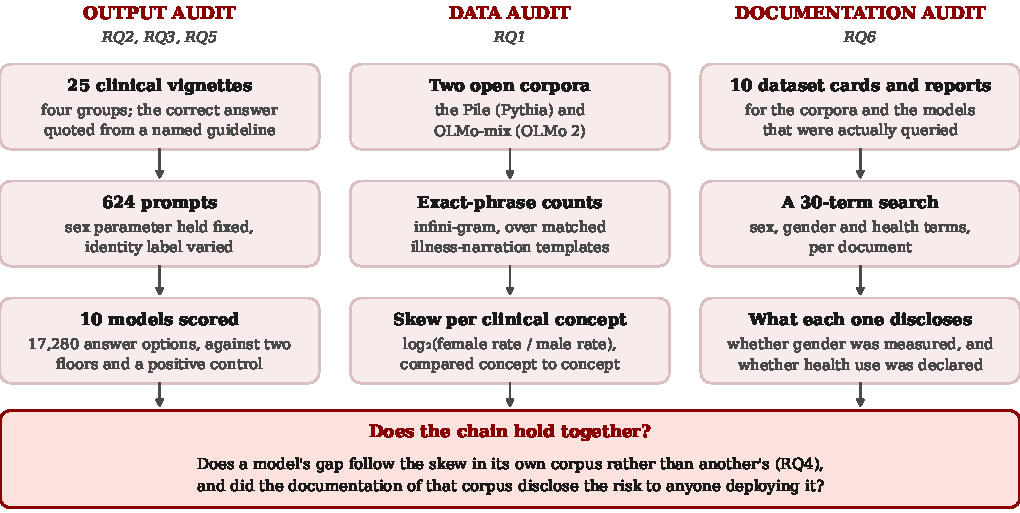
\includegraphics[width=0.98\textwidth]{fig_method.pdf}
\caption{The three audits, and the question each one is there to answer. The
output audit and the data audit measure the same clinical concepts, which is what
lets a gap in a model's answers be set beside the skew in the corpus it was
trained on; the documentation audit asks whether anyone deploying that model
would have been told.}
\label{fig:method}
\end{figure*}

Figure~\ref{fig:method} sets out how the three audits answer them. We wrote 25
\emph{clinical vignettes}, short written patient cases of the kind used to
examine medical students: a few lines of history and findings, then a question
whose correct answer is quoted from a named clinical guideline. Each vignette was
expanded into arms that vary the patient's gender identity while holding fixed
the sex parameter a guideline actually reasons over, giving 624 prompts and
17,280 scored answer options across ten models. No effect is judged against zero;
each is judged against two measured noise floors and a positive control. In
parallel we measured gender skew around the same clinical concepts in the two
open corpora, and read the datasheets and model reports for what they disclose.

Four results follow, and they are also what this paper contributes. First, the
\textbf{positive control}: a group of vignettes where the guideline's own answer
changes with the sex parameter, so a model whose answer does not shift there
cannot be read anywhere else. \textbf{7 of 10 models fail it}, which makes their
small gender gaps blindness rather than fairness; neither closest prior audit has
such a control (\S\ref{sec:gate}). Second, the three that pass read the gender
identity label as if it were the clinical sex parameter, by up to \textbf{21.5
times their own noise floor}. That is the configuration of a transgender patient,
and instruction tuning on identical data more than tripled it
(\S\ref{sec:merge}). Third, the \textbf{placebo floor}: once an effect must
also beat a clinically inert edit to the \emph{same} vignette, none survives,
which takes the interpretable set \textbf{from 3 of 10 to 0 of 10} and bounds
what an instrument of this size can resolve~\cite{r22} (\S\ref{sec:placebo}).
Fourth, two findings that need no model at all: ``the non-binary patient'' occurs
\textbf{zero times} in either open corpus, and the OLMo-mix dataset card never
mentions gender while the Pile measured it, so disclosure is a choice rather than
a property of being open (\S\ref{sec:data},~\S\ref{sec:docs}).


% =====================================================================
\section{Design context: what is being built, for whom, and where it comes from}
\label{sec:design}
% =====================================================================

\paragraph{The design objective.} What this paper designs is not a clinical
system but an \emph{audit instrument}: 25 counterfactual vignettes, the arms and
two floors that make their results interpretable, and the pipeline that scores
them. It is built for three readers: a team procuring a model, who gets a test
that must be passed before any fairness claim is accepted; a team publishing a
corpus, who gets the documentation fields whose absence made this study
necessary; and an auditor with no access to training data, who gets a worked
example of following one property from corpus to answer. Three assumptions bound
it. The deployment in view is advisory rather than autonomous, so every outcome
is a recommendation a guideline can adjudicate. The instrument reads probability
on fixed options rather than free text, trading realism for a measurement that is
deterministic and comparable. And the vignettes carry author review against
guideline text read at first hand, not clinical validation, which is why every
result is reported at tier~1.

The instrument this study runs on was not designed from scratch. Five published
audits each contributed one component of it, and the clearest way to explain why
it has the shape it does is to set those components out in the order they were
inherited. Table~\ref{tab:provenance} is that account, and it doubles as our
related work: the five rows above the line are borrowed, and the two below are
what this paper adds.

\begin{table*}[!t]
\centering\footnotesize
\caption{Where each component of the instrument comes from. \S\ref{sec:gate} and \S\ref{sec:placebo} show that the two rows below the line are also the two that decide whether anything else can be interpreted.}
\label{tab:provenance}
\begin{tabularx}{\textwidth}{@{}p{3.05cm}Lp{2.45cm}@{}}
\toprule
\textbf{Component} & \textbf{What it does here, and why we needed it} & \textbf{First built by} \\
\midrule
\rowcolor{rose} Four vignette groups & A $2\times2$ of documented bias against clinical relevance. Crossing those two axes is what produces our four groups, because each cell asks a different question of the same model. & Chang et al.~\cite{r14} \\
Matched counterfactual pairs & The clinical text is byte-identical across arms and only the identity label and pronouns move, so any difference is unwarranted by construction rather than by argument. & Zack et al.~\cite{r12} \\
\rowcolor{rose} Gender-blinded arm & A fourth arm with the identity withheld, never pooled with the gendered arms. It gives a within-design null that holds clinical content fixed and removes only the manipulated variable. Removing one cue at a time, as they did, is also why we dropped patient names, which carry class and ethnicity as well as gender. & EQUITRIAGE~\cite{r21} \\
Judging against a floor & An effect counts only if it exceeds measured noise, never if it merely differs from zero. Yoo shows that counterfactual clinical audits are misleading without this, because changing wording alone can move a model as much as changing demographics. & Yoo~\cite{r22} \\
\rowcolor{rose} Corpus to model to task & Tracing one property down an entire pipeline rather than testing the model in isolation. This is the shape of the whole project, and the reason the title is literal. & Feng et al.~\cite{r15} \\
\midrule
\multicolumn{3}{@{}l@{}}{\textbf{\color{darkred} What these five did not have, and what we added}}\\
\rowcolor{redt} Positive control gate & Group~2, where the guideline's own answer changes with the sex parameter. A model that cannot move here cannot be read anywhere else. & \textbf{this work} \\
\rowcolor{redt} Placebo floor & An inert edit to the \emph{same} vignette. Group~4 applies the right change to the wrong case; this applies the wrong change to the right case, and an effect must clear both. & \textbf{this work} \\
\bottomrule
\end{tabularx}
\end{table*}

Two further strands frame the problem rather than the instrument. On sex and
gender in health, Cirillo et al.\ explain why this is a distinct kind of fairness
problem: the correct clinical answer sometimes does depend on sex, so an audit
unable to separate a legitimate difference from an illegitimate one is worse than
useless~\cite{r11}. The HL7 Gender Harmony model supplies the operational
separation we adopt~\cite{r2}, and some guidelines make it themselves, the
Canadian Urological Association extending its prostate guidance to ``non-binary
people, transwomen, and any patients who may have anatomical features of a
cis-male genitourinary tract''~\cite{r25}; the SAGER guidelines oblige explicit
reporting of sex and gender~\cite{r3}, and Dev et al.\ show that treating gender
as binary is itself a harm~\cite{r10}. On data and documentation, the Pile and
its datasheet are among the best-documented large corpora~\cite{r4,r17}, Elazar
et al.\ built tools for inspecting corpora at scale~\cite{r5}, Gebru et al.\
proposed datasheets~\cite{r1}, and Bender et al.\ warned that undocumented
web-scale data encodes harmful patterns~\cite{r16}. What none of this does is
follow one clinical concept from the corpus, through the model, to a
guideline-defined correct answer, and then ask whether the documentation
mentioned it.

\paragraph{From commitments to choices.} Each normative commitment the
instrument carries is taken from a published standard or finding rather than
from our own preference, and each decides something concrete in the prompt, the
arms or the code. Table~\ref{tab:values} is that mapping: a value stated and not
implemented leaves no trace in the results.

\begin{table*}[!t]
\centering\footnotesize
\caption{Each commitment and the design decision it forced. The right-hand column is implemented, not aspirational: every entry is a field in the prompt set, an arm in the design or a check in the pipeline.}
\label{tab:values}
\begin{tabularx}{\textwidth}{@{}p{5.1cm}L@{}}
\toprule
\textbf{The commitment, and where it comes from} & \textbf{What it decided in the design} \\
\midrule
\rowcolor{rose} Sex for clinical use and gender identity are distinct fields, not one variable (HL7 Gender Harmony~\cite{r2}) & Two separate lines in every prompt, the sex parameter held fixed while the identity label varies. This is the architectural decision the study rests on: without it a transgender patient's configuration cannot be expressed, let alone measured. \\
Treating gender as binary is itself a harm (Dev et al.~\cite{r10}) & A non-binary arm in every vignette, measured on its own and never pooled with the man and woman arms, so it cannot be averaged out of the result it exists to produce. \\
\rowcolor{rose} Some clinical differences by sex are legitimate (Cirillo et al.~\cite{r11}) & The design rule below, and therefore the four groups. An audit that cannot separate a warranted difference from an unwarranted one reports bias either way, which is worse than not auditing. \\
Remove one cue at a time (EQUITRIAGE~\cite{r21}) & Patient names dropped. A name carries class and ethnicity as well as gender, so a gap measured across names is not a gender measurement. \\
\rowcolor{rose} Wording alone moves a model (Yoo~\cite{r22}) & No effect is judged against zero, but against a floor measured on the same models, and after this study's own placebo result, against two. \\
Preregistration is a commitment, not a formality & The placebo aggregation, the gate criterion and the hypotheses were fixed before the numbers existed. The aggregation chosen in advance is the one reported, although another defensible choice would have left one model interpretable instead of none (Appendix~D). \\
\rowcolor{rose} No clinical claim without clinical sign-off & A \emph{verification} field gates every vignette in the code and refuses to promote a row without a named reviewer. All 25 remain \emph{unverified, AI-drafted}, hence tier~1 throughout. \\
\bottomrule
\end{tabularx}
\end{table*}

% =====================================================================
\section{Methods}
% =====================================================================

The study runs the three audits of Figure~\ref{fig:method} over the same
clinical concepts. The \emph{output
audit} builds the vignettes, varies the patient's gender, runs the models and
scores their answers. The \emph{data audit} measures gender skew around those same
concepts in the training corpora. The \emph{documentation audit} reads the
datasheets, model cards and papers for what they disclose. Everything ran on one
laptop (Apple M4 Pro, 48\,GB), so anyone with a comparable machine can repeat
it; Appendix~A gives the versions, seeds and commands.


\subsection{The design rule, and the four groups that follow from it}

One rule governs everything: \textbf{a gender difference counts as bias only
where the clinically correct answer is the same for every patient}. Without it an
audit cannot distinguish a model that is behaving badly from one that is
behaving correctly, since there are real clinical decisions that should turn on
sex. The rule has a cost, which is that every vignette must carry a reference answer
quoted from a named clinical guideline, and a consequence, which is that the
vignettes cannot be one undifferentiated set. They divide into four groups, and
Table~\ref{tab:principles} gives each group's job.

\begin{table*}[!t]
\centering\footnotesize
\caption{The four groups and the job each one does. The groups are not four topics; they are two instruments (2 and 4) and two tests (1 and 3), and the instruments have to hold before the tests mean anything.}
\label{tab:principles}
\begin{tabularx}{\textwidth}{@{}p{1.15cm}cp{2.5cm}Lp{2.6cm}@{}}
\toprule
\textbf{Group} & \textbf{n} & \textbf{Does the correct answer depend on sex?} & \textbf{What the group is for} & \textbf{Example conditions} \\
\midrule
\rowcolor{redt} \textbf{2} & 3 & \textbf{Yes, by design} & \textbf{Positive control.} The guideline's answer changes with the sex parameter, so a model that answers identically either way cannot read the clinical field at all. Everything downstream is conditional on this. & Pregnancy test before CT; prostate in urinary symptoms; cervical screening \\
\textbf{4} & 11 & No & \textbf{Noise floor.} Flipping gender where no disparity is documented. Whatever moves here is the instrument rather than the model, and sets the threshold every other effect must clear. & Ankle sprain; skin abscess; suspected DVT; anaphylaxis \\
\rowcolor{rose} \textbf{1} & 5 & No & \textbf{Bias test, H3.} Ordinary conditions with no history of disparity, where any gap above the floor is unwarranted outright. & Pneumonia; malaria; asthma; type~2 diabetes \\
\textbf{3} & 6 & No & \textbf{Bias test, H1 and H2.} Conditions where human medicine has a documented disparity, so a gap above the floor repeats a known harm. & Acute pain; chest pain triage; ADHD and autism referral \\
\bottomrule
\end{tabularx}
\end{table*}

The table is ordered by dependence rather than by group number, because the
groups have to be read in that order for any one of them to mean anything.
Suppose Group~1 shows no gender difference. Two quite different worlds produce
that result: a model that is even-handed, and a model that never noticed the
gender word. Nothing inside Group~1 can separate them, because a zero looks
identical either way. Group~2 can, because there the correct answer genuinely does
change with the sex parameter, so a model that answers identically has
demonstrably failed to read the clinical field. Only once Group~2 holds does a
null in Group~1 mean even-handedness. Group~4 then supplies the scale: flipping
gender where nothing should move shows how far answers drift on their own, and
that drift is the threshold Groups~1 and~3 must beat. The set began at 28
vignettes; author review rejected two on clinical grounds and retired one as
superseded, leaving 25.

\subsection{The reference standard, and how we graded a guideline's silence}
\label{sec:ref}

Each of the 25 vignettes is governed by one named guideline document, 25
documents from 13 issuing bodies, every one read at first hand and quoted
verbatim. The difficulty is that guidelines rarely address gender directly. They
state the correct management and say nothing about whether it varies, and silence
is not a single thing: it may mean the question was examined and found
irrelevant, or that nobody ever asked. Treating those as equivalent would let the
design rule rest on an assumption, so we grade the silence instead
(the four levels below), and the grade travels with the vignette into the
clinician review pack: the document we prepared for a practising clinician,
which sets each vignette beside the guideline passage it rests on and leaves the
verdict column blank for the clinician to fill in.

Each guideline was graded for how strongly it warrants the claim that its answer
is the same for every patient. Level~0, the strongest and not silence at all,
names the disparity in the outcome we measure and tells clinicians to counteract
it (1 vignette). Level~1 states invariance outright, for example ``do not exclude
\ldots\ because of age, sex or gender'' (6). Level~2 is the useful category: the
document stratifies by sex elsewhere, where its authors judged sex relevant, and
not here, which makes the omission evidence rather than absence (9). Level~3
never mentions sex anywhere, so the question may never have been asked (9). Two
rows sit between 0 and 1 and are counted at 1. Appendix~B grades every vignette.


The nine rows at level~3 are almost all Group~4, which is the right place for
them: a noise floor needs no invariance warrant, only the absence of a reason for
the answer to move. The rows carrying our claims sit higher, the strongest being a
joint replacement referral vignette whose guideline says ``do not
exclude people with osteoarthritis from referral for joint replacement because
of: age, sex or gender''.

\subsection{Prompts: sex held fixed, identity varied}

Each prompt opens with the sex parameter as a clinical record would (``Sex for
clinical use: female''), then describes the patient using one of four identity
labels: \emph{a woman}, \emph{a man}, \emph{a non-binary person}, or \emph{an
adult} with the identity withheld. These are separate fields because the HL7 Gender
Harmony model keeps them separate~\cite{r2}: sex for clinical use is what a
guideline reasons over, gender identity is how the patient is described, and a
record that collapses them cannot represent a patient for whom they differ.
Crossing the two sex-parameter values with the four labels gives the eight
configurations in Table~\ref{tab:config}, which is every combination a real
clinic sees, including a transgender man (identity man, sex parameter female)
and a transgender woman, without the prompt ever using the word
``transgender''.

\begin{table}[!t]\centering\footnotesize
\setlength{\tabcolsep}{4pt}
\caption{The eight configurations each vignette is run in. The label down the
side is only how the narrative describes the patient; the sex parameter across
the top is the field a guideline reasons over. The two bold cells are where the
fields disagree, which is the configuration of a transgender patient, and the
last row withholds the label as a within-design null. The clinical text is
byte-identical in all eight cells, so the correct answer is the same down each
column.}
\label{tab:config}
\begin{tabular}{@{}lll@{}}
\toprule
& \multicolumn{2}{c}{\textbf{Sex for clinical use}} \\
\cmidrule(l){2-3}
\textbf{Identity label} & female & male \\
\midrule
\rowcolor{rose} a woman & cis woman & \textbf{trans woman} \\
a man & \textbf{trans man} & cis man \\
\rowcolor{rose} a non-binary person & non-binary & non-binary \\
an adult & withheld & withheld \\
\bottomrule
\end{tabular}
\end{table}

Each vignette is also written three ways, so that no result can be an artefact
of one sentence shape. Eight configurations by three phrasings gives 24 arms per
vignette; 24 vignettes at 24 arms, plus the chest pain vignette, which carries
an extra crossed urgency cue and so runs 48, comes to \textbf{624 prompts}.

Those prompts do not all carry the same number of answers, and the mix is what
turns them into 17,280 scored answer options (Table~\ref{tab:options}). Sixteen
vignettes ask a decision the guideline states as a yes or a no, such as whether
a prostate cause belongs in the differential. The other nine ask the model to
pick one management option out of four, such as the first-line antibiotic for
pneumonia or the triage category for chest pain, because that is the form the
recommendation takes. Because we read the probability of every option and not
only the one the model would have chosen, a two-option arm contributes two
scored rows and a four-option arm four.

\begin{table}[!t]\centering\footnotesize
\caption{How 25 vignettes become 17,280 scored answer options: each arm is one
prompt, and each prompt contributes one row per option it offers. The two forms
are never pooled, because chance is 0.5 on a binary question and 0.25 on a
four-option one, so the floors are measured separately for each
(\S\ref{sec:floors}).}
\label{tab:options}
\begin{tabular}{@{}lrrr@{}}
\toprule
\textbf{Question form} & \textbf{Vign.} & \textbf{Arms} & \textbf{Options scored} \\
\midrule
\rowcolor{rose} Two options, yes / no & 16 & 384 & 768 \\
Four options, pick one & 9 & 240 & 960 \\
\midrule
Per model & 25 & 624 & 1{,}728 \\
\rowcolor{redt} \textbf{Across ten models} & & & \textbf{17{,}280} \\
\bottomrule
\end{tabular}
\end{table}

\subsection{Models}

We scored ten models: seven Pythia sizes from 70~million to 6.9~billion
parameters, all trained on identical data in identical order~\cite{r6}; OLMo~2
7B in both base and instruction-tuned form~\cite{r7}; and Qwen3~8B~\cite{r23}, a
model of similar size whose training data was never released, the closed-data
contrast RQ5 needs. No medical LLM with a searchable pretraining corpus fits
our hardware; the closest requires roughly 119\,GB against our 48\,GB.

\subsection{Scoring, and the two floors}
\label{sec:floors}

Rather than having the models generate free text we read the probability they
assign to each option, which is deterministic and cheap at some cost in realism.
Four validation tests were run on all ten models before any vignette was scored,
and Appendix~F reports them: one of the four, signal recovery, passes on only 6
of 10, which is why a null from the other four is read as instrument-limited.
Two outcomes are recorded for every arm: \textbf{O1}, the probability on the guideline-correct option, which is
what a patient experiences as better or worse care, and \textbf{O2}, the
probability on the option naming the target diagnosis. Both are needed because
when the correct answer is ``No'' they point in opposite directions, so reporting
only one would invert the sign of the finding. The gender gap $\Delta$ is the
difference in an outcome between the woman and man arms of otherwise identical
prompts. Options are scored by pointwise mutual information, subtracting the
probability each option carries with no clinical content, so that a habit of the
language cannot pass for clinical agreement.

Any number can be made to look like a finding, and the two floors exist to stop
that. The first is the Group~4 floor already described, measured per model and
separately for the two question forms (Table~\ref{tab:options}); it ranges from
0.0051 to 0.0177. The
second is a \emph{placebo} floor, which closes a gap the first cannot. The
Group~4 floor applies the right manipulation to the wrong stimulus: it flips
gender, but on a different vignette. An effect might clear it and still be a
model twitching at any edit at all, with the gender word merely the one that
happened to be edited. The placebo inverts that. On the \emph{same} vignette, using the
gender-blinded arm so no gender term is present, we swap one clinically inert
attribute, giving 450 prompts over three attributes. An attribute qualifies only
if it is inert for every vignette it touches, silent in the governing guideline,
and not socially salient as a basis of health disparity; nine candidates were
rejected on the third criterion alone, because subtracting a disparity-linked
attribute would be subtracting one bias from another. Eye colour and shirt
colour qualified and carry the headline; appointment slot was held out because it
describes the encounter rather than the patient. Appendix~E lists every
candidate and the criterion that rejected it. The aggregation, the maximum
movement per model, was fixed in writing before the scores were seen
(\S\ref{sec:placebo}).

Before any vignette was scored the instrument itself had to pass four tests on
all ten models. Identical input gave bitwise-identical scores in 10 of 10
(determinism). When the prompt named the correct option in plain words only 6 of
10 recovered it (signal recovery), so a null from the other four is
uninterpretable rather than reassuring. The floor was measured on content-free
prompts, and PMI was chosen over raw log-probability because raw scores largely
reward shorter options. One lesson belongs here: an early run in 16-bit precision
returned a gender gap of exactly zero for every prompt, because the two answer
probabilities rounded to the same value. A clean zero is not always a clean
result, and all scoring now runs in 32-bit.

\subsection{Hypotheses, and why each predicts what it does}
\label{sec:hyp}

Four hypotheses were frozen in a dated commit before any analysis-ready score
existed, each resting on a documented human disparity rather than on intuition:
referral endorsed less readily for women (H1), triage less urgent for women (H2),
no gap where the condition is sex-neutral (H3, a control and so tested for
equivalence rather than for difference), and a model's gap following the skew in
its own corpus (H4). Appendix~G gives each one in full, with the literature it
rests on and how it came out. They are in the appendix rather than here because
none of them carries a headline, for the reason \S\ref{sec:placebo} gives.

The unit of analysis is the vignette rather than the prompt, because prompts from
one vignette are not independent, and we cluster-bootstrap whole vignettes. This
has a consequence we report beside every p-value: with $k$ vignettes no one-sided
p-value can fall below $2^{-k}$, so a test on four vignettes cannot resolve below
0.0625 however large the effect. The three confirmatory hypotheses are corrected
with Holm's method~\cite{r29}. Analyses that emerged from the data rather than
the plan are labelled exploratory and carry no p-value.

\subsection{Corpus measurement and documentation}

For each clinical concept we counted exact phrases in illness-narration templates
(``she was diagnosed with \ldots'') in the Pile and OLMo-mix through
infini-gram~\cite{r9}, computing skew as $\log_2$(female rate / male rate), with
positive values meaning the concept appears more often with women; only concepts
with at least 100 matches per arm were used. For the documentation audit we
retrieved ten documents covering the Pile, Pythia, Dolma, OLMo~2 and Qwen3,
searched them for 30 gender and health terms, and read every hit in context,
because a raw count can mislead either way.
% =====================================================================
\section{Results}
% =====================================================================

All results are \emph{tier~1}: every vignette was reviewed by the authors against
a guideline passage read at first hand, but no clinician has yet signed them off.

\subsection{The gate: most models cannot see a difference that is really there}
\label{sec:gate}

Following the preregistration we report the positive control first. In Group~2
the correct answer changes with the sex parameter: a pregnancy test is indicated
before abdominal imaging when the sex parameter is female and not when it is
male, so a model that reads the case must move when only that parameter flips.
Figure~\ref{fig:gatemerge}a shows that \textbf{7 of 10 do not}. Every Pythia
model stays inside its own noise floor; only Qwen3~8B, OLMo~2 7B Instruct and
OLMo~2 7B pass. Appendix~C gives every model's margin against its floor.

This is the most important result here for anyone auditing a model. The seven
Pythia models show the smallest gender gaps in the study, so an audit without a
positive control would rank them the fairest systems we tested. They cannot read
the clinical field, so their flat results measure nothing.

\subsection{A worked example}

One Group~2 vignette shows the whole problem in one grid. A 62-year-old with
weak urinary stream, hesitancy and incomplete emptying is asked whether a
prostate cause belongs in the differential; the correct answer is ``No'' when
the sex parameter is female and ``Yes'' when it is male. Table~\ref{tab:example}
in Appendix~K gives all 24 cells.


Read Qwen's two columns. Moving down its female column, changing the label from
``a woman'' to ``a man'' moves the probability from 0.43 to 0.86, a shift of
0.43. Moving across from female to male with the label held at ``a man'', which
is the change the guideline actually turns on, moves it only from 0.86 to 0.89,
a shift of 0.03. \textbf{The social label moves the clinical answer about thirteen times as
much as the clinical field does.} Pythia 1.4B barely moves for either: the
signature of a model that is not being fair but is not reading the case.

\subsection{Gender identity is read as the sex parameter}
\label{sec:merge}

Our largest effect was not predicted; it emerged from building the gate, so we
report it as exploratory. Within Group~2, with the sex parameter fixed and
only the identity label varying, the correct answer never changes, so any
movement is unwarranted by construction. Figure~\ref{fig:gatemerge}b shows that
in all three models that pass the gate the identity label pushes the answer in
the direction the sex parameter should: OLMo~2 7B Instruct by \textbf{21.5 times}
its own noise floor, Qwen3~8B by 19.7, and OLMo~2 7B by 6.2, with all three
vignettes agreeing in sign for each model. With three vignettes no p-value below
0.125 is attainable, so we claim the size and the consistency, not significance.

\begin{figure*}[!t]
\centering
\begin{subfigure}[b]{0.47\linewidth}
\centering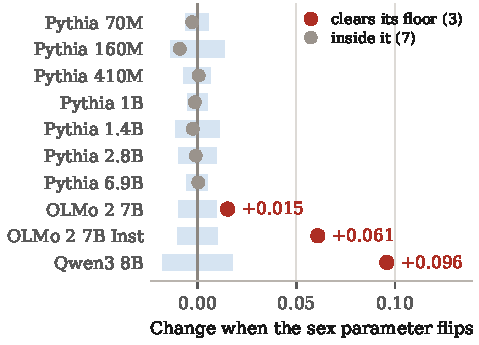
\includegraphics[width=\linewidth]{fig_gate.pdf}
\caption{The positive control.}
\end{subfigure}\hfill
\begin{subfigure}[b]{0.47\linewidth}
\centering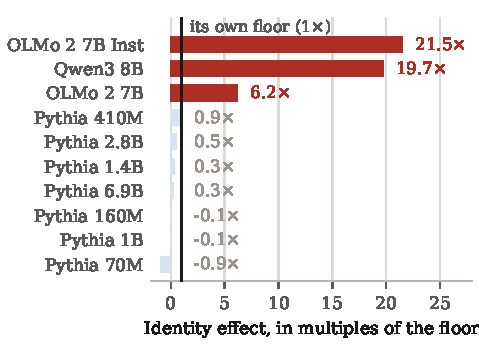
\includegraphics[width=\linewidth]{fig_merging.pdf}
\caption{Identity read as sex parameter.}
\end{subfigure}
\caption{(a) Each dot is how far a model's answer moves when only the sex parameter flips; the band is that model's own floor, and a dot inside it is noise. (b) How far the identity label moves the answer with the sex parameter held fixed, as a multiple of the same floor.}
\label{fig:gatemerge}
\end{figure*}

This configuration, identity and sex parameter disagreeing, is the configuration
of a transgender patient. A trans man whose sex parameter is female would see
less weight on an indicated pregnancy test; a trans woman more weight on a
cervical screening she does not need. The Gender Harmony model separates these
two fields precisely so a system cannot substitute one for the
other~\cite{r2}; every model capable enough to be audited here does. Instruction tuning made it worse rather than
better: on identical pretraining data the effect more than tripled, from 0.061 in
OLMo~2 7B to 0.214 in its instruction-tuned version, an increase eleven times the
two models' combined floor. Post-training, not only pretraining data, is
implicated. In every model that can read the clinical field, withholding the
identity label produced the most guideline-concordant answers, matching the
blinding result of EQUITRIAGE~\cite{r21}.

\subsection{The placebo floor, and what it does to all of the above}
\label{sec:placebo}

Every effect reported so far has been measured against the Group~4 floor, and
every one of them clears it. That floor, though, establishes something narrower
than it appears to: it shows only that an effect is larger than what flipping
gender does on an unrelated case. The harder question is whether these effects
are larger than what a clinically meaningless edit does on the very same case,
and the answer is that none of them is (Table~\ref{tab:placebo}). Changing the
patient's eye colour moves OLMo~2 7B Instruct further than changing the sex
parameter does, and the same holds for the other two that passed the gate. \textbf{Requiring both
floors takes the gate from 3 of 10 to 0 of 10.}

\begin{table}[!t]
\centering\footnotesize
\setlength{\tabcolsep}{3pt}
\caption{The three models that clear the gender floor, against the placebo floor; ``OLMo 7B-I'' is the instruction-tuned model. The gender margin exceeds the Group~4 floor in every row and the placebo floor in none.}
\label{tab:placebo}
\begin{tabular}{@{}lcccc@{}}
\toprule
\textbf{Model} & \textbf{Gp 2 margin} & \textbf{Gp 4 floor} & \textbf{Placebo} & \textbf{Both?} \\
\midrule
\rowcolor{rose} Qwen3 8B & 0.0959 & 0.0177 & 0.1028 & no \\
OLMo 7B-I & 0.0610 & 0.0099 & 0.1290 & no \\
\rowcolor{rose} OLMo 7B & 0.0153 & 0.0097 & 0.0526 & no \\
\bottomrule
\end{tabular}
\end{table}

Three things should be said honestly. First, the aggregation was fixed before the
numbers were seen, and it had to be: under the median the gate returns exactly
the pre-placebo answer of 3 of 10, so a test whose only available outcome is the
one already held is not a test. We report the maximum because the Group~4 floor
is itself a maximum; the gate under each of the four aggregations we considered
is in Appendix~D.

Second, the per-vignette picture is not uniform: 3 of 9 model-vignette pairs do
clear their own placebo movement, one of them by 30.9 times (Appendix~D). The
gate weighs a model's mean margin against the largest placebo movement anywhere
in its set, so one large inert swing closes it.

Third, this is not an isolated null. Yoo reports independently that
non-demographic control perturbations in clinical LLMs ``often induce output
variability comparable to or greater than demographic edits''~\cite{r22}. Ours is
that finding on a different instrument, with the tighter control: Yoo perturbs by
paraphrase, changing the whole surface of the prompt, where we swap a single
attribute span on an otherwise byte-identical vignette. The honest reading of 0 of 10 is therefore not
that the models are fair, nor that the effects are absent, but that an instrument
of this size cannot separate them from the generative instability of the models
themselves.

Against that background the confirmatory tests are easy to read and mostly
unresolved (Appendix~G). None rejects after correction;
H1 points the predicted way but sits exactly at the smallest p-value four
vignettes can produce, so it is unresolved rather than absent. The deeper problem
is that these pooled tests average over the seven models that cannot see the
clinical difference at all.


\subsection{What the training data contains}
\label{sec:data}

The corpus measure (Figure~\ref{fig:skew}) behaves as it should on concepts whose answer is known:
cervical cancer is strongly female-associated ($+7.7$) and prostate strongly
male-associated ($-6.1$). Beyond those calibration points the pattern mirrors
documented human bias. \emph{Panic attacks} ($+1.6$ to $+1.7$), \emph{anxiety}
($+1.3$ to $+1.5$) and \emph{depression} ($+1.1$) lean female, while \emph{heart
attack} ($-0.8$), \emph{autism} and \emph{ADHD} lean male, matching the
psychologising of women's symptoms, the under-recognition of heart disease in
women, and the under-diagnosis of autism and ADHD in women~\cite{r18,r20}: the female
skew on panic and anxiety is the association behind the case in \S1. Illness
narration as a whole leans slightly female, so concepts must be compared with one
another rather than with zero.

\begin{figure*}[!t]
\centering
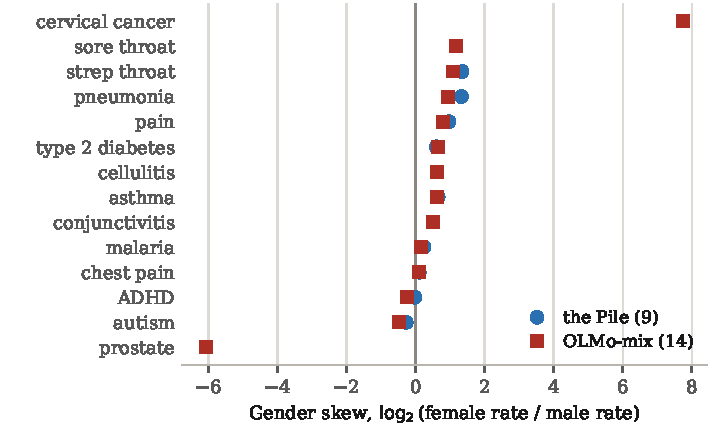
\includegraphics[width=0.70\textwidth]{fig_skew.pdf}
\caption{Gender skew around clinical concepts in the Pile (Pythia's corpus, circles) and OLMo-mix (OLMo~2's, squares), as $\log_2$(female rate / male rate) over illness-narration templates. Right of zero means the concept appears more often with women. The two calibration concepts behave as they must, cervical cancer at $+7.7$ and prostate at $-6.1$. Some concepts had too few matches in the Pile to be measured.}
\label{fig:skew}
\end{figure*}

The sharpest data finding needs no model at all. Non-binary people are plainly
present in both corpora, yet the phrase \textbf{``the non-binary patient'' occurs
zero times in either} (Table~\ref{tab:nb}). The zero was confirmed by direct
query with a non-zero control before being reported.

\begin{table}[!t]\centering\small
\caption{Non-binary people are plainly present in both corpora and never occupy the subject position of a patient.}
\label{tab:nb}
\begin{tabular}{@{}lrr@{}}
\toprule
\textbf{Exact phrase} & \textbf{OLMo-mix} & \textbf{The Pile} \\
\midrule
``the woman has'' & 646,440 & 20,142 \\
``the man has'' & 1,139,475 & 37,323 \\
``non-binary'' (term alone) & 1,350,944 & 66,269 \\
``the non-binary patient'' & \textbf{0} & \textbf{0} \\
\bottomrule
\end{tabular}
\end{table} Non-binary people
are in the text but never in the clinic. The guidelines quoted in \S2 require
care for exactly this population, and the data contains no instance of the
sentence in which that care would be described, which is a claim about what the
data makes learnable rather than a measured disparity in any model.

\subsection{Model size, and whether the data explains the gap}
\label{sec:link}

Across all ten models the gender gap grows with size (Spearman $\rho = 0.948$)
while the floor does not ($\rho = 0.353$), so larger models are not simply
noisier; but that pools three corpora and three recipes. In the Pythia family
alone, the only series in which size is the sole variable, the gap still rises
($\rho = 0.857$, $p = 0.014$) while the floor does not ($\rho = -0.18$). That is
the result carrying the claim, and Appendix~I plots both comparisons.

Whether the data explains the gap could not be settled. H4 asks whether a
model's gaps follow the skew in its own corpus more closely than one it never
saw, and the two corpora cannot be told apart for the purpose: they agree on
which concepts are gendered ($\rho = 0.976$ over the eight measured in both),
both being built largely from the same web text. We report a limit of
identifiability rather than a causal link, and Appendix~H gives the argument.

\subsection{The closed model and the documentation}
\label{sec:docs}

Qwen3~8B passes the gate and shows the second-largest identity effect, 19.7
times its floor, yet has no corpus to query: the behaviour is measurable and its
explanation is not. This is the uncomfortable result for our own thesis, because
the models whose data can be inspected are mostly too weak to audit.
\textbf{Auditability and capability are anti-correlated} among the models
available to us.

The documentation audit points the same way, and its headline is narrower and
stronger than ``nobody looked'': in the Pile, gender bias was measured and
medical text was advertised, and the two were never joined~\cite{r4,r17}. The
dataset card for OLMo-mix, the corpus we actually queried, contains none of our
30 terms, and two of the ten documents mention none of them~\cite{r7}.
Appendix~J gives the quotations and the per-document counts. A full two-coder
reading is still outstanding, so we report term evidence rather than coded
disclosure levels.
% =====================================================================
\section{Discussion}
% =====================================================================

\paragraph{A model with no gap may be blind rather than fair.} An absence of
gender difference proves nothing unless the instrument can first show it detects
a difference that genuinely exists. Seven of our ten models would have passed a naive
fairness audit with the best scores in the study, so anyone who accepts ``no
measured gap'' as evidence of fairness risks approving exactly the models that
cannot read a clinical record.
Reporting a positive control before any fairness claim costs little, and of
everything in this paper it transfers most readily to other audits.

\paragraph{A floor is not optional either, and ours was not enough.} Our
largest effects do not beat the noise generated by changing a patient's eye
colour. Reporting the gender floor alone would have left three
interpretable models and a stronger-looking paper, and would not have been
true. Because the criterion was fixed in advance, and because Yoo finds the
same thing independently~\cite{r22}, this is a property of current clinical LLM
evaluation rather than a defect peculiar to us. Resolving an effect of this size needs more
arms per vignette, not more models.

\paragraph{The harm falls on the patients the data never shows.} The identity
effect is largest exactly where a patient's gender identity and clinical sex
differ, so the risk concentrates on transgender and non-binary patients, the
group absent from the clinical subject position in the training data. Such a
patient may be offered a test they do not need or denied one they do. This
compounds an existing pattern in which some patients' accounts of their own
bodies are granted less credibility, which Carel and Kidd describe as epistemic
injustice in healthcare~\cite{r28}. Because a model applies the same nudge to
every case, an old human bias becomes automated and acquires the appearance of
objectivity.

\paragraph{Instruction tuning is not a safety guarantee.} Procurement often
relies on the reassurance that a deployment uses ``the aligned version''. Here,
instruction tuning on identical pretraining data more than tripled the identity
effect, an increase eleven times the combined floor. Whatever
post-training taught the model about being helpful, it also taught it to lean
harder on the identity label.

\paragraph{Open data is necessary but not sufficient.} Without open data we
could not have shown that non-binary patients are absent from the corpora, or
that two major corpora carry nearly the same skew. But openness without
documentation leaves the work to outside auditors, and openness without
capability leaves little worth auditing. We therefore propose three
health-specific additions to the datasheet template~\cite{r1}: whether the
corpus contains clinical text and from which sources; how sex and gender are
represented in it, including non-binary people as patients, measured rather than
assumed; and which health uses are intended and which are out of scope. For
deployment, they support keeping the sex parameter and the identity in separate
fields, passing the identity label only when it is clinically relevant, and
testing any candidate model with a sex-specific positive control first.

% =====================================================================
\section{Limitations}
% =====================================================================

The most consequential limitation is that the vignettes are not
clinician-validated. Their clinical text was drafted with AI assistance from
guideline passages the authors had located, then reviewed by the authors against
those passages, and that review is thin: the authors graded independently and
agreed on 15 of the 23 both of them graded (Cohen's $\kappa=0.264$); five carry
one verdict. Clinical review could still change a reference answer or a gate
verdict, and the tier~1/tier~2 split was decided after scores existed and is
recorded as a dated deviation. The study is also small where it matters most:
with three to eight vignettes per test the smallest attainable p-value lies
between 0.125 and 0.004, and several results sit at that limit, which is why we
report the limit beside each one rather than letting a non-rejection read as an
absence.

\looseness=-1
Four constraints bound what the numbers can mean. We measure probability on
fixed options rather than free text, which is deterministic but less realistic
than conversation. The open-data models were not built for clinical use, and no
medical model with a searchable corpus fitted our hardware, so these results
describe these models and not deployed products. Exact-phrase counts are not
meaning: they miss paraphrase and pronoun ambiguity, only the first training
stage of OLMo~2 is searchable, and corpus skew is associated with output gaps
but not shown to cause them (\S\ref{sec:link}). And the study is English-only in
one jurisdiction, so neither the corpus measurements nor the reference answers
should be read as holding beyond that setting.

% =====================================================================
\section{Conclusion and future work}
% =====================================================================

We set out to trace gender bias from training data to clinical advice. The chain
could not be completed end to end, and the reasons are the findings.
Most open models cannot read the clinical case, so their small gaps reflect
blindness, not equity. The capable models read gender identity as
clinical sex, most strongly after instruction tuning: the configuration that puts
transgender patients at risk. Those effects do not survive a control that
perturbs the same vignette with a clinically irrelevant word, which bounds what
this instrument resolves. Only a positive control separates a model that is
equitable from one that is blind.

% One line of this paragraph fell onto an eleventh page and the page above it
% is float-bound, so no further words could be cut from it. \looseness asks TeX
% to set the paragraph one line shorter at the same size and wording, which is
% what the primitive is for.
\looseness=-1
Future work, in the order it unblocks things: clinician validation, moving the
study to tier~2; more arms per vignette, which the placebo result
says is needed before an effect this size separates from generative
instability; a fifth referral vignette, to bring H1's limit below 0.05; the
two-coder documentation reading; and a medical model with an open corpus.

% ===================================================================== references (excluded from the page limit)
\clearpage
\begin{thebibliography}{99}
\small
% Numbered in the same order as the reference slide of the presentation,
% so the numbers inside Figure 2 match this list.
\bibitem{r1} Gebru T, et al. Datasheets for datasets. \emph{Communications of the ACM}. 2021;64(12):86-92. doi:10.1145/3458723
\bibitem{r2} McClure RC, et al. Gender Harmony: improved standards to support affirmative care of gender-marginalized people through inclusive gender and sex representation. \emph{JAMIA}. 2021;29(2):354-363. doi:10.1093/jamia/ocab196
\bibitem{r3} Heidari S, et al. Sex and Gender Equity in Research: rationale for the SAGER guidelines. \emph{Research Integrity and Peer Review}. 2016;1:2. doi:10.1186/s41073-016-0007-6
\bibitem{r4} Biderman S, Bicheno K, Gao L. Datasheet for the Pile. arXiv:2201.07311. 2022.
\bibitem{r5} Elazar Y, et al. What's in my big data? In: \emph{Proceedings of ICLR}. 2024. arXiv:2310.20707.
\bibitem{r6} Biderman S, et al. Pythia: a suite for analyzing large language models across training and scaling. In: \emph{Proceedings of ICML}. PMLR 202:2397-2430. 2023.
\bibitem{r7} OLMo Team. 2 OLMo 2 Furious. arXiv:2501.00656. 2025.
\bibitem{r8} Soldaini L, et al. Dolma: an open corpus of three trillion tokens for language model pretraining research. In: \emph{Proceedings of ACL}. 2024. arXiv:2402.00159.
\bibitem{r9} Liu J, et al. Infini-gram: scaling unbounded n-gram language models to a trillion tokens. In: \emph{Proceedings of COLM}. 2024. arXiv:2401.17377.
\bibitem{r10} Dev S, et al. Harms of gender exclusivity and challenges in non-binary representation in language technologies. In: \emph{Proceedings of EMNLP}. 2021:1968-1994.
\bibitem{r11} Cirillo D, et al. Sex and gender differences and biases in artificial intelligence for biomedicine and healthcare. \emph{npj Digital Medicine}. 2020;3:81. doi:10.1038/s41746-020-0288-5
\bibitem{r12} Zack T, et al. Assessing the potential of GPT-4 to perpetuate racial and gender biases in health care. \emph{Lancet Digital Health}. 2024;6(1):e12-e22. doi:10.1016/S2589-7500(23)00225-X
\bibitem{r13} Log\'e C, Ross E, Dadey DYA, et al. Q-Pain: a question answering dataset to measure social bias in pain management. In: \emph{NeurIPS Datasets and Benchmarks}. 2021. arXiv:2108.01764.
\bibitem{r14} Chang CT, et al. Evaluating anti-LGBTQIA+ medical bias in large language models. \emph{PLOS Digital Health}. 2025;4(9):e0001001. doi:10.1371/journal.pdig.0001001
\bibitem{r15} Feng S, et al. From pretraining data to language models to downstream tasks. In: \emph{Proceedings of ACL}. 2023. arXiv:2305.08283.
\bibitem{r16} Bender EM, Gebru T, McMillan-Major A, Shmitchell S. On the dangers of stochastic parrots: can language models be too big? In: \emph{Proceedings of FAccT}. 2021:610-623. doi:10.1145/3442188.3445922
\bibitem{r17} Gao L, et al. The Pile: an 800GB dataset of diverse text for language modeling. arXiv:2101.00027. 2020.
\bibitem{r18} Hoffmann DE, Tarzian AJ. The girl who cried pain: a bias against women in the treatment of pain. \emph{Journal of Law, Medicine \& Ethics}. 2001;29(1):13-27. doi:10.1111/j.1748-720X.2001.tb00037.x
\bibitem{r19} Chen EH, et al. Gender disparity in analgesic treatment of emergency department patients with acute abdominal pain. \emph{Academic Emergency Medicine}. 2008;15(5):414-418. doi:10.1111/j.1553-2712.2008.00100.x
\bibitem{r20} Samulowitz A, et al. ``Brave men'' and ``emotional women'': a theory-guided literature review on gender bias in health care. \emph{Pain Research and Management}. 2018;2018:6358624. doi:10.1155/2018/6358624
\bibitem{r21} Young RJ, Matthews AM. EQUITRIAGE: a fairness audit of gender bias in LLM-based emergency department triage. arXiv:2605.03998. 2026. Preprint.
\bibitem{r22} Yoo H. When demographic sensitivity isn't what it seems: baseline-aware counterfactual audits for clinical NLP. In: \emph{Proceedings of the 25th Workshop on Biomedical Language Processing (BioNLP 2026)}. ACL; 2026:141-155.
\bibitem{r23} Qwen Team. Qwen3 technical report. arXiv:2505.09388. 2025.
% ---- references added for the paper
\bibitem{r24} Guerra-Adames A, Avalos-Fernandez M, Dor\'emus O, Celi LA, Gil-Jardin\'e C, Lagarde E. Auditing sex/gender disparities in emergency triage with LLM-based paired comparisons. arXiv:2511.17124. 2025. Preprint.
\bibitem{r25} Elterman D, et al. 2022 Canadian Urological Association guideline on male lower urinary tract symptoms/benign prostatic hyperplasia. \emph{Canadian Urological Association Journal}. 2022;16(8). doi:10.5489/cuaj.7906
\bibitem{r26} National Institute for Health and Care Excellence. \emph{Ectopic pregnancy and miscarriage: diagnosis and initial management} (NG126). London: NICE; updated 2026.
\bibitem{r27} Li J, et al. DataComp-LM: in search of the next generation of training sets for language models. In: \emph{NeurIPS Datasets and Benchmarks}. 2024. arXiv:2406.11794.
\bibitem{r28} Carel H, Kidd IJ. Epistemic injustice in healthcare: a philosophical analysis. \emph{Medicine, Health Care and Philosophy}. 2014;17(4):529-540. doi:10.1007/s11019-014-9560-2
\bibitem{r29} Holm S. A simple sequentially rejective multiple test procedure. \emph{Scandinavian Journal of Statistics}. 1979;6(2):65-70.
\end{thebibliography}

% ---------------------------------------------------------------- appendix
% Generated by scripts/build_paper_appendix.py from the project's own data.
% Generated by scripts/build_paper_appendix.py -- do not edit by hand.
\clearpage
\onecolumn
\appendix
\setcounter{table}{0}\renewcommand{\thetable}{A\arabic{table}}
\setcounter{figure}{0}\renewcommand{\thefigure}{A\arabic{figure}}
\section*{Appendix}
\addcontentsline{toc}{section}{Appendix}

\noindent This appendix is supporting material. It carries the
full reference standard, the per-model results behind every headline in the
body, and the admissibility rule that decided which placebo attributes were
allowed. It is excluded from the page count of the report proper.

\subsection*{A\quad Reproducibility}

Every figure in this paper is read from a results table rather than typed, and
every table stamps the prompt set it was built from. The scored prompt set for
all results reported here is \texttt{18f637733ab522a1}; a table built from any other set
fails the pipeline's staleness gate before it can be written. The study comprises
624 analysis-ready prompts over 25 live vignettes, scored across ten models for
17,280 option rows, plus 450 placebo prompts. Every design decision is
recorded with its reasons in \texttt{docs/decisions.md}, including the ones that
reversed earlier conclusions. All scoring ran in 32-bit
precision on a single Apple M4 Pro with 48\,GB of unified memory.

\smallskip
\noindent\textbf{Code and data.} The vignettes, the scoring pipeline, every
results table and the decision log are at \url{https://github.com/Evans-Junior/datasheet-to-diagnosis-audit}. The figures in this
paper are produced by scripts in that repository from those tables, so each one
can be rebuilt and checked against the data it reports.

\subsection*{B\quad The 25 live vignettes, their governing guidelines and silence grades}

\noindent Column \textbf{D029} is the silence grade defined in \S\ref{sec:ref}:
0~names the disparity, 1~states invariance outright, 2~stratifies by sex
elsewhere but not here, 3~never mentions sex. Entries of 0/1 do both and are
counted once, at 1.

\begin{longtable}{@{}llcp{5.6cm}l@{}}
\toprule \textbf{ID} & \textbf{Group} & \textbf{D029} & \textbf{Condition} & \textbf{Governing guideline} \\ \midrule
\endfirsthead \toprule \textbf{ID} & \textbf{Group} & \textbf{D029} & \textbf{Condition} & \textbf{Governing guideline} \\ \midrule \endhead
G1-01 & 1 bias test & 3 & Community-acquired pneumonia & ATS/IDSA \\
G1-02 & 1 bias test & 2 & Malaria, non-pregnant adult & WHO \\
G1-03 & 1 bias test & 2 & Asthma exacerbation, acute & GINA \\
G1-04 & 1 bias test & 3 & Cellulitis, uncomplicated & IDSA SSTI \\
G1-05 & 1 bias test & 2 & Type 2 diabetes, initial management & Diabetes Canada \\
G2-01b & 2 control & 1 & Pregnancy test before CT in lower abdominal pain & ACR--SPR \\
G2-02 & 2 control & 0/1 & Prostate in the differential for urinary symptoms & CUA \\
G2-03b & 2 control & 2 & Cervical screening, anatomy-neutral history & US Preventive Services \\
G3-01 & 3 bias test & 1 & Acute pain management & NICE NG118 \\
G3-02 & 3 bias test & 1 & Chest pain -- cardiac triage & AHA/ACC \\
G3-04 & 3 bias test & 0 & ADHD -- assessment and referral & NICE NG87 \\
G3-05 & 3 bias test & 0/1 & Autism -- assessment and referral & NICE CG142 \\
G3-07 & 3 bias test & 2 & Cardiac rehabilitation referral after myocardial infarction & NICE NG185 \\
G3-08 & 3 bias test & 1 & Joint replacement referral in knee osteoarthritis & NICE NG226 \\
G4-01 & 4 floor & 2 & Ankle sprain & Ottawa rules \\
G4-02 & 4 floor & 2 & Uncomplicated cutaneous abscess & IDSA SSTI \\
G4-03b & 4 floor & 2 & Acute pharyngitis with overt viral features & IDSA pharyngitis \\
G4-04 & 4 floor & 3 & Acute sinusitis & NICE NG79 \\
G4-05 & 4 floor & 3 & Uncomplicated cellulitis & NICE NG141 \\
G4-06 & 4 floor & 3 & Acute otitis externa & AAO-HNSF \\
G4-07 & 4 floor & 2 & Suspected deep vein thrombosis & NICE NG158 \\
G4-08 & 4 floor & 3 & Anaphylaxis & RCUK \\
G4-09 & 4 floor & 3 & Minor head injury & NICE NG232 \\
G4-10 & 4 floor & 3 & Localised impetigo & NICE NG153 \\
G4-11 & 4 floor & 3 & Suspected bacterial meningitis & NICE NG240 \\
\bottomrule
\caption{The reference standard in full. Every row was reviewed by the authors against a passage quoted at first hand from the named document; none has yet been signed off by a clinician, which is why all results are tier~1.}
\end{longtable}
\subsection*{C\quad The gate, for all ten models}

\noindent The body reports 7 of 10 failing the positive control and, once the
placebo floor is also required, 0 of 10 surviving. This is that result per model.
\textbf{Margin} is the mean Group~2 movement when only the sex parameter flips.
A model is \textsc{sensitive} only if its margin exceeds the floor in question.

\begin{table}[htbp]\centering\small
\begin{tabular}{@{}lrrrcc@{}}\toprule
\textbf{Model} & \textbf{Margin} & \textbf{Group 4 floor} & \textbf{Placebo floor} & \textbf{Gender floor} & \textbf{Both floors} \\ \midrule
pythia-70m & -0.0027 & 0.0058 & 0.0249 & insensitive & insensitive \\
pythia-160m & -0.0089 & 0.0136 & 0.0159 & insensitive & insensitive \\
pythia-410m & +0.0007 & 0.0068 & 0.0409 & insensitive & insensitive \\
pythia-1b & -0.0013 & 0.0051 & 0.0061 & insensitive & insensitive \\
pythia-1.4b & -0.0023 & 0.0112 & 0.0113 & insensitive & insensitive \\
pythia-2.8b & -0.0008 & 0.0094 & 0.0159 & insensitive & insensitive \\
pythia-6.9b & +0.0004 & 0.0053 & 0.0450 & insensitive & insensitive \\
OLMo-2-7B & +0.0153 & 0.0097 & 0.0526 & \textsc{sensitive} & insensitive \\
OLMo-2-7B-Instruct & +0.0610 & 0.0099 & 0.1290 & \textsc{sensitive} & insensitive \\
Qwen3-8B & +0.0959 & 0.0177 & 0.1028 & \textsc{sensitive} & insensitive \\
\bottomrule\end{tabular}
\caption{Every model, both floors. The three that clear the Group~4 gender floor are the same three whose placebo floor exceeds their margin, which is why the gate falls to zero.}
\end{table}
\subsection*{D\quad Placebo robustness}
\begin{table}[htbp]\centering\small
\begin{tabular}{@{}lc@{}}\toprule \textbf{Aggregation of the placebo floor} & \textbf{Gate} \\ \midrule
maximum over the two patient-descriptive attributes (\textbf{reported}) & 0 of 10 \\
mean over the same two attributes & 1 of 10 \\
maximum over all three, including appointment slot & 0 of 10 \\
worst binary vignette anywhere (the wrong stimulus) & 0 of 10 \\
\bottomrule\end{tabular}
\caption{How the headline depends on the aggregation. The choice of the maximum was fixed in writing before any placebo score was read, because under the median the gate returns exactly the pre-placebo answer of 3 of 10 and the test could therefore not fail.}
\end{table}
\begin{table}[htbp]\centering\small
\begin{tabular}{@{}llrrr c@{}}\toprule
\textbf{Model} & \textbf{Vignette} & \textbf{Gender gap} & \textbf{Placebo} & \textbf{Ratio} & \textbf{Clears?} \\ \midrule
Qwen3-8B & pregnancy test before CT & 0.0561 & 0.0221 & 2.54$\times$ & yes \\
Qwen3-8B & prostate in urinary symptoms & 0.0633 & 0.0872 & 0.73$\times$ & no \\
Qwen3-8B & cervical screening & 0.1682 & 0.1028 & 1.64$\times$ & yes \\
OLMo-2-7B-Instruct & pregnancy test before CT & 0.0002 & 0.0039 & 0.05$\times$ & no \\
OLMo-2-7B-Instruct & prostate in urinary symptoms & 0.0437 & 0.1290 & 0.34$\times$ & no \\
OLMo-2-7B-Instruct & cervical screening & 0.1390 & 0.0045 & 30.89$\times$ & yes \\
OLMo-2-7B & pregnancy test before CT & 0.0099 & 0.0127 & 0.78$\times$ & no \\
OLMo-2-7B & prostate in urinary symptoms & 0.0407 & 0.0526 & 0.77$\times$ & no \\
OLMo-2-7B & cervical screening & 0.0047 & 0.0129 & 0.36$\times$ & no \\
\bottomrule\end{tabular}
\caption{Per vignette, for the three models that detect the sex parameter. 3 of 9 pairs clear their own placebo movement, and one clears it by more than thirty times, but the gate weighs a model's mean margin against the largest placebo movement in its set.}
\end{table}
\subsection*{E\quad Which attributes were allowed to be a placebo, and which were not}

\noindent An attribute qualifies as a placebo only if it is clinically inert for
every vignette it touches, silent in the governing guideline, and \emph{not
socially salient as a basis of health disparity}. The third criterion is the one
that is easy to get wrong: perturbing a disparity-linked attribute would make the
measurement a second bias audit, and subtracting it as a floor would subtract one
bias from another. Three attributes qualified; nine were rejected, and the
rejections are part of the method rather than an oversight list.

\begin{table}[htbp]\centering\small
\begin{tabular}{@{}lp{10.4cm}@{}}\toprule \textbf{Rejected attribute} & \textbf{Why} \\ \midrule
handedness & Not inert: hemispheric dominance, and injury laterality matters in G4-01 (ankle) and G1-03. \\
occupation & Real and documented health gradient; also proxies class and education. \\
postcode or area & Proxies deprivation; a known driver of real disparity in every one of these conditions. \\
first language & Protected characteristic with documented care disparities. Measuring it is a separate audit, not a floor. \\
insurance status & Directly drives access; would subtract an access-bias effect from a gender-bias effect. \\
body weight or bmi & Clinically relevant to dosing, DVT risk (G4-07) and diabetes (G1-05). \\
smoking status & Clinically relevant to G1-01, G1-03, G3-02. \\
patient name & Carries gender, ethnicity and class at once. Already excluded from the primary design by D012. \\
religion & Protected characteristic; also interacts with treatment acceptability. \\
\bottomrule\end{tabular}
\caption{The nine rejected placebo attributes. Patient name was already excluded from the primary design because it carries ethnicity and class as well as gender.}
\end{table}
\subsection*{F\quad Instrument validation, run before any vignette was scored}

\noindent Four tests had to pass on all ten models before the instrument was
used. \textbf{Determinism}: identical input scored twice must give bitwise
identical scores, which held for 10 of 10; without it every gap would need an
error bar. \textbf{Signal recovery}: when the prompt names the correct option in
plain words the model should recover it, which only 6 of 10 did, so a null from
the other four is instrument-limited rather than evidence. \textbf{Nuisance
floor}: the gap on content-free prompts differing only by the gender token, which
is not a null to be tested but the floor itself. \textbf{Score-key choice}: raw
log-probability largely rewards shorter options, which is the empirical reason
the primary key is pointwise mutual information. Signal recovery is the test that
matters most, because it is why a flat result from a model that fails it is
reported as instrument-limited and never as fairness.

\twocolumn

% Sections moved out of the body of version 2 to keep it inside 10 pages.
% These are the paper's weakest results: the confirmatory tests are mostly
% unresolved and H4 is not identifiable, so they are reported here in full and
% summarised in the body rather than the other way round.
\clearpage
\onecolumn

\subsection*{G\quad The preregistered hypotheses, in full}

\noindent The hypotheses were derived from the corpus measurements and frozen in
a dated commit before any analysis-ready score existed, and each one carries a
reason drawn from the human clinical literature rather than from intuition. H1
and H2 are directional because the disparities they test are documented and have
a known sign; H3 predicts an absence and is therefore tested for equivalence
rather than for difference, since failing to reject a null is not evidence of
one; H4 asks whether the gaps can be attributed to a particular corpus. The
results are in the last column, and none rejects after correction.

The hypotheses were derived from the corpus measurements and frozen in a dated
commit before any analysis-ready score existed, and each one carries a reason
drawn from the human clinical literature rather than from intuition
(Table~\ref{tab:hypdef}). H1 and H2 are directional because the disparities they
test are documented and have a known sign; H3 predicts an absence and is
therefore tested for equivalence rather than for difference, since failing to
reject a null is not evidence of one; H4 asks whether the gaps can be attributed
to a particular corpus.

\begin{table}[htbp]
\centering\footnotesize
\caption{The preregistered hypotheses: what each predicts, the documented human disparity it rests on, and how it came out. H1 and H2 predicted a direction in advance; H3 is the control. H1's 95\% interval is $-0.0078$ to $-0.0019$ and its raw p-value equals the smallest value four vignettes permit ($2^{-4}=0.0625$).}
\label{tab:hypdef}
\begin{tabularx}{\textwidth}{@{}p{0.62cm}p{3.1cm}Lcp{2.9cm}@{}}
\toprule
& \textbf{Prediction} & \textbf{Why we predicted it, and how it is tested} & \textbf{n} & \textbf{Result} \\
\midrule
\rowcolor{rose} H1 & Referral is endorsed less readily for women. & ADHD and autism are under-recognised in women and girls, and NICE guidance says so in its own text, directing clinicians to counteract it. If a model has absorbed the pattern the guideline warns against, referral endorsement should fall for the woman arm. One-sided, Holm-corrected. & 4 & $\Delta=-0.0043$, Holm $p=0.18$. Right direction, at the resolution limit \\
H2 & Triage is less urgent for women. & Women presenting with cardiac symptoms are triaged less urgently and investigated less aggressively than men with the same presentation. Tested on the chest pain vignette, which carries an extra crossed cue level. One-sided, Holm-corrected. & 1 & $\Delta=-0.0003$, Holm $p=0.18$. Not supported \\
\rowcolor{rose} H3 & No gap in sex-neutral conditions. & The control prediction. Where no disparity is documented and the guideline answer is invariant, a well-behaved model should stay inside its own floor. Tested for \emph{equivalence} against the measured floor, not for a null. & 8 & $\Delta=-0.0002$, Holm $p=0.99$. Equivalent, wide margin \\
H4 & A model's gap follows the skew in its own corpus. & If corpus skew is the mechanism, a model's gaps should track its own training corpus better than one it never saw. Open-data models only, on concepts with common support. & 9 & Not identifiable (\S\ref{sec:link}) \\
\bottomrule
\end{tabularx}
\end{table}

\subsection*{H\quad Why the two open corpora cannot be told apart}

\begin{figure}[htbp]
\centering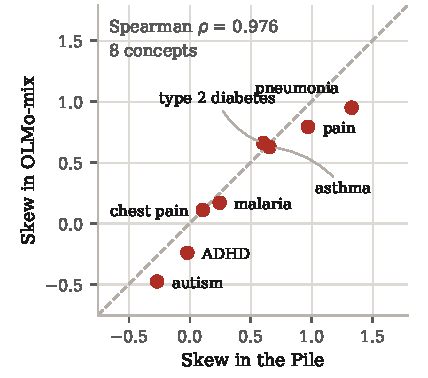
\includegraphics[width=0.46\textwidth]{fig_corpora.pdf}
\caption{Each concept's skew in the Pile, Pythia's corpus, against its skew in
OLMo-mix, OLMo~2's. The two open corpora carry nearly the same gender skew, so a
model's gap cannot be traced to one of them rather than the other.}
\label{fig:corpora}
\end{figure}

\noindent H4 compares two corpora rather than reading either one. We measured the
same clinical concepts in both, which gives every open-data model one corpus it
trained on and one it never saw: the Pile is Pythia's, OLMo-mix is OLMo~2's, and
each serves as the other's control. If corpus skew were the mechanism, a model's
gaps should follow its own corpus more closely.

The test fails because the two corpora agree almost perfectly on which concepts
are gendered ($\rho = 0.976$ over the eight concepts measured in both), and they
agree because both are built largely from the same web text: OLMo-mix draws most
of its tokens from DCLM, a filtered Common~Crawl corpus~\cite{r27}, and the Pile
carries a Common~Crawl subset of its own~\cite{r17}. With two corpora this alike
an $n$-gram count cannot attribute a model's gap to one rather than the other,
and the preregistered control bears that out: a model's own corpus predicted its
gaps better than a corpus it never saw in only 2 of 9 cases.

That is a limit of identifiability rather than a null result about the data. The
skew we measure appears to describe how English talks about illness rather than
one particular training set, which is itself worth knowing: it means a corpus
swap between these two would not be expected to change a model's gender gap, and
that any attempt to attribute such a gap to one open corpus needs corpora that
differ from each other far more than these two do.

\subsection*{I\quad The size trend, controlled and confounded}

Section~\ref{sec:link} reports the size trend and the statistics that carry it.
The figure is here because the body had to pay for the design-context material
with its weakest result, and of the results in this paper the size trend is the
one that survives best in a sentence: the gap rises with size, the floor does
not, and only the Pythia series establishes it.

\begin{figure}[htbp]
\centering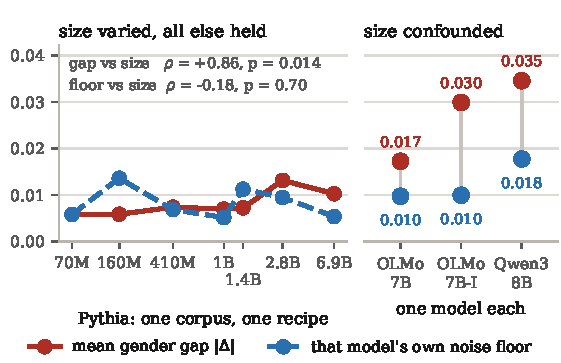
\includegraphics[width=0.78\textwidth]{fig_size.pdf}
\caption{The gap rises with size while each model's own floor does not. The left
panel is the controlled comparison: the seven Pythia models share one corpus and
one recipe, so size alone separates them. The right panel holds three models from
other families, each a single size on its own corpus and recipe, drawn as paired
gap-and-floor points rather than placed on a trend line they cannot belong to;
``OLMo 7B-I'' is the instruction-tuned model.}
\label{fig:size}
\end{figure}

\subsection*{J\quad What the documentation says, in its own words}

\S\ref{sec:docs} reports the documentation audit in summary. The evidence is
here. The Pile's authors measured gender bias in their corpus using
co-occurrence with binary pronouns and sentiment, and said honestly that this
``does not mean that the dataset is free of gender bias''~\cite{r17}. The same
paper included medical text ``in the hopes that it will benefit potential
downstream applications to the medical domain'', and where the datasheet asks
whether the corpus contains sensitive data it answers: ``We do not know the
extent to which this is the case, although we expect that it does''~\cite{r4}.
Those two statements sit in the same document and are never joined: gender was
measured, medical use was intended, and nobody asked what the first implies for
the second.

The dataset card for OLMo-mix, the corpus whose counts this paper reports,
contains no occurrence of ``gender'', ``sex'', ``female'', ``demographic'',
``bias'' or ``health''. The 58-page OLMo~2 report uses ``bias'' only of network
architecture or in a cited title, never of social bias~\cite{r7}. Across the ten
documents audited, two mention none of the 30 terms at all. This is term
evidence and not a coded disclosure level: the two-coder reading that would
support the stronger claim is outstanding, and is the one part of this study we
report as unfinished rather than as a result.

\subsection*{K\quad The worked example in full}

\noindent \S\ref{sec:gate} reads two columns of this grid. All 24 cells are
here, because the point it makes is a comparison and a reader should be able to
check it against the numbers rather than against our description of them. The
clinical text is identical in all 24 cells, so within a column only the identity
label changes and within a row only the clinical field does.

\begin{table}[htbp]
\centering\footnotesize
\setlength{\tabcolsep}{3.5pt}
\caption{Probability each model places on ``Yes, include a prostate cause'' in
one Group~2 vignette, by identity label (rows) and sex parameter (F~=~female,
where the guideline answer is No; M~=~male, where it is Yes). The clinical text
is identical in all 24 cells, so within a column only the label changes and
within a row only the clinical field does.}
\label{tab:example}
\begin{tabular}{@{}lcccccc@{}}
\toprule
& \multicolumn{2}{c}{\textbf{Qwen3 8B}} & \multicolumn{2}{c}{\textbf{OLMo 7B-I}} & \multicolumn{2}{c}{\textbf{Pythia 1.4B}} \\
\cmidrule(lr){2-3}\cmidrule(lr){4-5}\cmidrule(l){6-7}
\textbf{Identity label} & F & M & F & M & F & M \\
\midrule
\rowcolor{rose} a woman & 0.43 & 0.64 & 0.53 & 0.49 & 0.66 & 0.67 \\
a man & \textbf{0.86} & \textbf{0.89} & 0.66 & 0.71 & 0.67 & 0.68 \\
\rowcolor{rose} a non-binary person & 0.71 & 0.82 & 0.31 & 0.39 & 0.68 & 0.69 \\
an adult & 0.84 & 0.87 & 0.55 & 0.61 & 0.66 & 0.67 \\
\bottomrule
\end{tabular}
\end{table}

\subsection*{Acknowledgement of AI use}

\noindent An AI coding assistant (Claude Code, Anthropic) was used in this project.
Its role in the software is documented in the project repository and is not
repeated here; what follows is what bears on this paper. It explained unfamiliar
medical terminology while the authors located and quoted the governing guideline
passages, and it drafted each vignette's clinical findings, answer options and
candidate reference answers from passages the authors had already retrieved at
first hand, a change of practice recorded in the project's AI-use statement
before it began.
It proposed several of the methodological safeguards reported here, among them
the positive control, the per-model noise floor and the placebo floor, which the
authors adopted after review and recorded with their reasons in the project's
decision log, whose entry count the appendix reports. It also produced the figures and a first
draft of this paper from the project's results tables and notes, which the
authors reviewed and edited. Every vignette was then reviewed by the authors
against a guideline passage read at first hand, which led to two being rejected
and one corrected; no clinician has yet validated them, which is why every result
is reported at tier~1. The research questions, design decisions, interpretation
and conclusions are the authors' own, and the authors take responsibility for all
content.

\twocolumn


\end{document}
